\documentclass[12pt]{article}
\parindent0em
\parskip 1ex plus 0.4ex minus 0.4ex

\usepackage[a4paper,vmargin=30mm,hmargin=25mm]{geometry}
\usepackage{polyglossia}
\setdefaultlanguage{german}
\usepackage{fontspec}
\usepackage{lipsum}
\usepackage{xcolor}
\usepackage{listings}
\usepackage{graphicx}

\definecolor{lstbackground}{rgb}{0.95,0.95,1}      % hellgruener Rahmen
\lstset{language=Python}

\lstset{
  basicstyle=\small\ttfamily,
  backgroundcolor=\color{lstbackground},
  keywordstyle=\bfseries\ttfamily\color{blue},
  stringstyle=\color{orange!50!black}\ttfamily,
  commentstyle=\color{gray}\ttfamily,
  showstringspaces=false,
  flexiblecolumns=false,
  tabsize=4,
  numbers=left,
  numberstyle=\tiny,
  numberblanklines=true,
  stepnumber=1,
  numbersep=10pt,
  xleftmargin=15pt,
  literate=%
  {Ö}{{\"O}}1
  {Ä}{{\"A}}1
  {Ü}{{\"U}}1
  {ß}{{\ss}}1
  {ü}{{\"u}}1
  {ä}{{\"a}}1
  {ö}{{\"o}}1
  {~}{{\textasciitilde}}1
}

\begin{document}

\begin{center}
  \textbf{\LARGE Sichere Programmierung} \\[1ex]%
  \textbf{\Large Projekt 2}\\[1ex] %
  \textbf{\Large Einführung in Python}\\[3ex] %
  Nils Klein \\ %
  (79373) \\[1ex] %
  Alexander Krause \\ %
  (79878) \\[1ex] %
  Abdullah Yildiz \\ %
  (79669) \\[1ex] %
  Dozentin: Corina Hampel \\%
  
\end{center}


\newpage
\setcounter{page}{2}
\tableofcontents

\newpage
\section{Teil 1: GDB Aufgabe 1}
\subsection{Teil A - Analyse des Codes}
Das Skript \textbf{"gdb-uebung-1.c"} enthält nur eine main() Methode. Es wird die Bibliothek \textbf{"stdio.h"} importiert, und vorerst nur eine vorzeichenlose Ganzzahl Variable \textbf{"i"} deklariert:

\begin{lstlisting}
    #include <stdio.h>
    
    int main(){
        unsigned int i;
        ..
        ..
    }
\end{lstlisting}

Die Bibliothek \textbf{"stdio.h"} bietet mehrere Funktionen für Kommandozeilen Inputs / Outputs an. Darunter fällt auch \textbf{"printf"} das im weiteren Verlauf des Codes verwendet wird.\\
Durch den Datentyp \textbf{"unsigned"} kann kein Überlauf der Zahlen von Positiv auf Negativ erfolgen. Bei einem signed int ist der maximale Wert "2147483647". Sobald nun um eins erhöht wird entsteht ein Überlauf, und es ist der Wert -2147483648 vorhanden. Durch \textbf{unsigned} int sind ausschließlich positive Zahlen möglich (0 - 4294967295).\\
Der kurze Code besitzt auch die folgende for-Schleife:\\

\begin{lstlisting}
    for(i=0; i<20; i++){
        printf("i: %2d\n", i);
    }
\end{lstlisting}

Die for-Schleife initialisiert als erstes \textbf{"i"} mit dem Wert "0". Die Bedingung der for-Schleife lautet, solange \textbf{i} kleiner als \textbf{20} ist, soll die Schleife ausgeführt werden. In der Schleife wird durch \textbf{printf} die Variable \textbf{i} auf der Kommandozeile ausgegeben. Die Funktion besteht aus einem Formatierungsteil und den konkret auszugebenden Argumenten. In den Anführungszeichen wird ein String angegeben, der zusätzlich folgendes Argument \textbf{"\%2d\textbackslash n"} enthält. Das Argument ist für die Ausgabe von zweistelligen Integer-Werten verantwortlich. Nach dem Formatierungsteil wird durch ein \textbf{","} getrennt der Wert der Variable \textbf{"i"} angegeben.\\
Nach diesen Erkenntnissen wird in jedem Schleifendurchlauf die Variable \textbf{i} solange jeweils immer um 1 erhöht und ausgegeben, bis sie die Zahl 20 erreicht. Ist der Wert 20 erreicht wird die Schleife und damit auch das Programm beendet:\\
\begin{lstlisting}
    return 0;
\end{lstlisting}
\newpage

\subsection{Teil B - Kompilieren des Programms}

In Aufgabe 1b soll das Programm \textbf{gdb-uebung1.c} ausgeführt werden. Nach dem Kompilieren und starten wird folgendes ausgegeben:
\\
\begin{figure}[htbp]
    \centering
    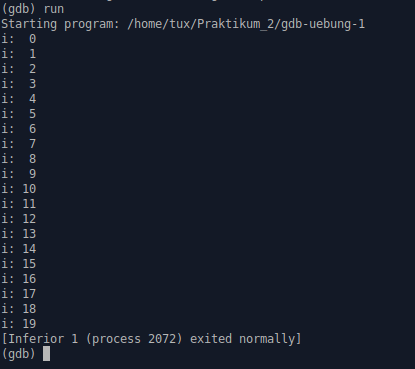
\includegraphics[width=16cm]{Praktikum 2/Bilder/1b_run}
    \caption{Aufgabe 1b, Ausgabe des Terminals}
    \label{fig:Uebung1b}
\end{figure}

Wie erwartet wird die Variable \textbf{"i"} von \textbf{0} bis inkl. dem Wert \textbf{19} ausgegeben, und bei \textbf{i = 20} das Programm beendet.
\newpage

\subsection{Teil C - Disassembly}
In dieser Teilaufgabe soll nun erklärt werden, wie der Maschinencode genau aufgebaut ist:\\
Der folgende Assemblercode kann in drei Abschnitte zerlegt werden:\\

\begin{figure}[htbp]
    \centering
    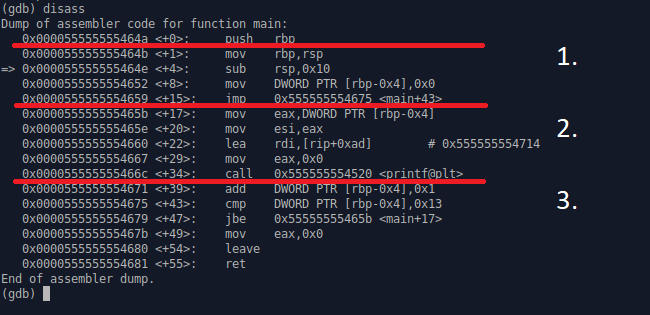
\includegraphics[width=16cm]{Praktikum 2/Bilder/1c_disass_3}
    \caption{Aufgabe 1c, Assemblercode}
\end{figure}

Im \textbf{ersten Abschnitt (1.)} ist die Initialisierung der Variable i und die for-Schleife enthalten.\\
Die erste wichtige Zeile ist die Initialisierung der Variable i die in Zeile 8 ("<+8>") stattfindet. Dort wird die Variable im Stack mit dem \textbf{DWORD} Wert \textbf{0x0} angelegt. Der Datentyp "DWORD" ist ein 32-Bit unsigned Integer. Wird der Hexadezimalwert 0x0 in das Dezimalsystem umgerechnet, entspricht das dem Wert 0, d.h. \textbf{i} ist jetzt mit dem Standardwert 0 deklariert.\\
Der Kopf der for-Schleife ist in Zeile 15 (<+15>) zu finden. Dort ist der Befehl \textbf{"jmp"} zu sehen, dadurch springt der Instruction Pointer (also der Pointer auf die Zeile, die aktuell ausgeführt wird) auf Zeile <+43> und vergleicht mittels dem Befehl \textbf{"cmp"} (compare) die Variable \textbf{i} mit dem Wert \textbf{"0x13"}. Der Dezimalwert der Hexadezimalen Zahl "0x13" entspricht 19. In der nächsten Zeile 47 wird auf die Zeile 17 "gesprungen", falls die Zahl kleiner oder gleich 19 ist. Dafür ist der Befehl \textbf{"jbe"} (Jump if Below or Equal) verwantwortlich. Laut der Doku sollte dieser Befehl verwendet werden, wenn man eine unsigned Integer Zahl vergleicht.\\
Im \textbf{zweiten Abschnitt} ist der Inhalt der for-Schleife, also die printf-Funktion, enthalten. Für die Funktionalität der Schleife ist das aber weniger relevant, weswegen hier nicht näher darauf eingegangen wird.\\
Im \textbf{dritten Abschnitt} ist das Erhöhen der Variable i und der Vergleich der for-Schleife (Also die Schleifenbedingung) vorhanden. Für das Erhöhen von i ist die Zeile 39 mit dem Befehl \textbf{"add"} verantwortlich. Hier wird der Wert \textbf{0x1} (also der Wert "1") zu dem Zieloperand "i" (im Register [rbp-0x4]) addiert.
Wie bereits erwähnt, wird der Vergleich in Zeile 43 durch \textbf{"cmp"} vorgenommen. Es wird der Inhalt von DWORD PTR [rbp-0x4] mit dem Wert 0x13 (Dec: 19) verglichen.
Ist die Zahl größer als 0x13, wird die Schleife verlassen (leave) und danach das Programm beendet (ret).\\



\subsection{Teil D - GDB}

Für diese Aufgabe wurde die Intel-Notation verwendet. Um nun das Programm zu übersetzen sind folgende Befehle nötig:\\

\begin{lstlisting}
    gcc -g -c gdb-uebung-1.c
    gcc -o gdb-uebung-1 gdb-uebung-1.c
\end{lstlisting}

\begin{itemize}
  \item Der erste Parameter \textbf{"-g"} erzeugt beim Übersetzen des Programms Debug Informationen.
  \item Der zweite Parameter \textbf{"-c"} gibt den Pfad zur Quelldatei an.
  \item Der dritte Parameter \textbf{"-o"} gibt den Dateinamen der neuen Datei an, die erstellt wird. Dadurch kann das Programm mit dem Namen \textbf{"gdb-uebung-1"} aufgerufen werden.
\end{itemize}

Nun kann der GNU-Debugger (GDB) verwendet werden:\\

\begin{lstlisting}
    gdb gdb-uebung-1
\end{lstlisting}

Die folgenden Befehle wurden in dieser Aufgabe verwendet:

\begin{itemize}
    \item b main
    \item run main
    \item disass
\end{itemize}

\begin{lstlisting}
b main = erzeugt einen Breakpoint am Anfang der Funtkion "main()".

run main = die Funktion main() wird ausgeführt.

disass = "disassembly", zerlegt eine Funktion oder einen Teil einer
         Funktion in Assemblercode.
    
nexti = führt die Zeile aus, auf die der Instruktion Pointer zeigt
        und setzt diesen eine Zeile weiter.
            
print i = gibt den Wert der Variable "i" aus.
    
quit = gdb verlassen.
\end{lstlisting}

\newpage
Nach einem b main, run main und letztlich \textbf{disass} entsteht folgender Output:

\begin{figure}[htbp]
    \centering
    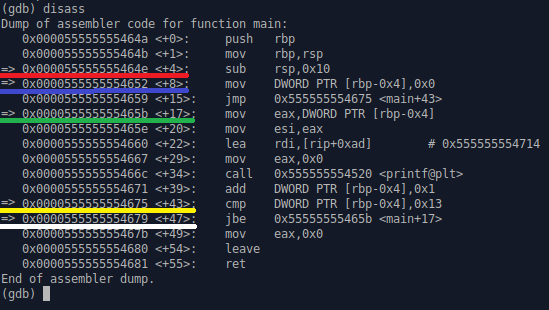
\includegraphics[width=16cm]{Praktikum 2/Bilder/1c_disass_photoshopskill9000.png}
    \caption{Aufgabe 1d, Assemblercode - "disass"}
\end{figure}

Der Pfeil links ist der \textbf{"Instruction Pointer"} und zeigt auf den Befehl der als nächstes ausgeführt wird. Auf diesem Bild ist der Instruction Pointer öfter zu sehen, weil das Bild bearbeitet wurde um nicht das gleiche Bild mehrmals zu verwenden. Natürlich ist der Instruction Pointer in einem disass-Output nur einmal vorhanden.\\

In den ersten drei Zeilen werden die Adressen des Stack-Frames initialisiert (\textbf{rote Linie}). \\

Durch den Befehl \textbf{"nexti"} wird der nächste Befehl ausgeführt. In Zeile acht findet somit die Initialisierung der Variable \textbf{"i"} mit dem Wert "0" statt (\textbf{blaue Linie}).\\


Als nächstes wird die Variable \textbf{i} mit dem Hexadezimalwert \textbf{"0x13"} in Zeile 43 verglichen (\textbf{gelbe Linie}).
Rechnet man die Hexadezimalzahl in eine Dezimalzahl um, ergibt sich die Zahl 19.\\

Falls die Zahl kleiner oder gleich 19 ist (jbe), wird in die Zeile 17 (<+17>) gesprungen \textbf{grüne Zeile}.\\

Nun wird erneut geprüft ob i kleiner oder gleich 19 ist (\textbf{weiße Linie}). Die Ausgaben werden bis i<20 ausgegeben (siehe Abbildung 1). Sobald i den Wert 20 erreicht, wird das Programm beendet.\\
\newpage

\section{Teil 2: GDB Aufgabe 2}
\subsection{Teil A - Analyse des Codes}

Das Skript \textbf{"gdb-uebung-2.c} enthält drei Funktionen und eine main() Methode. Es wird die Bibliothek \textbf{"stdio.h"} importiert:

\begin{lstlisting}
#include <stdio.h>

int f(int a, int b) {
  return 3*a + 7*b;
}

int g(int a, int b) {
  return 10*a*a - 3*b;
}

int h(int a, int b) {
  return a + b + 300;
}

int main() {
  int a = 5, b=9, c=0;

  c = f(g(a,h(a,b)),h(b,a));

  printf("a = %d, b = %d, c = %d\n", a, b, c);
}
\end{lstlisting}

In Zeile 18 wird in die Variable "c", der Wert eines geschachtelten Funktionsaufrufs gespeichert. Im Anschluss werden alle Variablen auf der Kommandozeile ausgegeben. Jedoch gibt es kein "return 0" in dem Quellcode.
\newpage

\subsection{Teil B - Kompilieren des Programms}

Die Ausgabe der Variablen a,b und c sollten folgende Werte haben:

\begin{itemize}
  \item a = 5
  \item b = 9
  \item c = 122
\end{itemize}
Die zwei Variablen a und b sind nicht weiter zu erklären. Das Ergebnis von c leitet sich aus der Verschachtelung ab:

\begin{itemize}
  \item Zu erst wird h(a,b) aufgerufen. Ergebnis = 314
  \item Als nächstes wird g(a, 317) aufgerufen. Ergebnis = -692
  \item Als nächstes wird h(b, a) aufgerufen. Ergebnis = 314
  \item Als letztes wird nun f(-692, 314) aufgerufen. Ergebnis = 122
\end{itemize}

Das Ergebnis ist wie erwartet:

\begin{figure}[htbp]
    \centering
    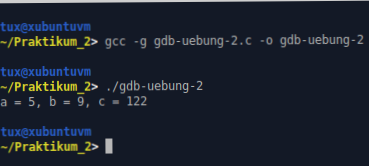
\includegraphics[width=10cm]{Praktikum 2/Bilder/2b_run_script.png}
    \caption{Aufgabe 2b, Ergebnis}
\end{figure}
\newpage

\subsection{Teil C - Disassembly}

\begin{itemize}
  \item In welcher Reihenfolge werden die Funktionen aufgerufen?
  \end{itemize}
  Das Programm ruft (Befehl: \textbf{call}) zuerst die Funktion h(a,b) einmal auf \textbf{(1)}. Durch die Verschachtelung wird die Funktion h(b,a) erneut aufgerufen mit verdrehten Parametern \textbf{(2)}. Danach kommt die Funktion g(a,h(a,b)) \textbf{(3)} und als letztes die Funktion f(g(a,h(a,b)),h(b,a)) \textbf{(4)}.
  
\begin{figure}[htbp]
    \centering
    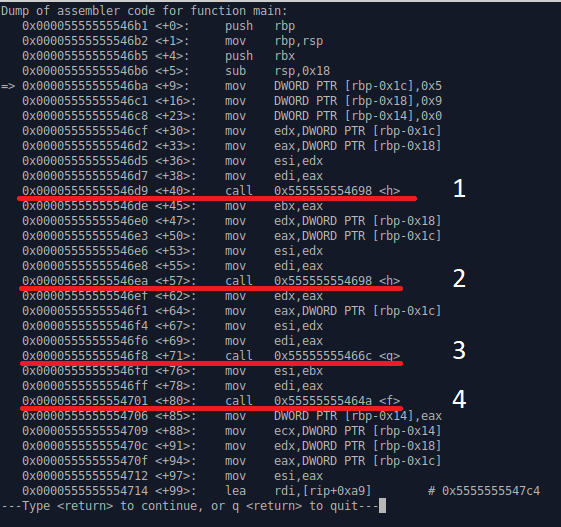
\includegraphics[width=16cm, height=10cm]{Praktikum 2/Bilder/2c_reihenfolge.png}
    \caption{Aufgabe 2c, Reihenfolge der aufrufe}
\end{figure}
  
\begin{itemize}
  \item Welche Stack Frames werden erzeugt?
\end{itemize}
Es wird ein Stack Frame für die main() (Zeile <+0>) und eines für die anderen Funktionen (Zeile <+4>) erzeugt. Somit werden insgesamt zwei Frames per \textbf{push} erzeugt.
\newpage

\begin{itemize}
  \item Was ist der Inhalt der Stack Frames?
\end{itemize}
Durch \textbf{"info frame"} können Informationen \& Inhalt der Frames angezeigt werden:
\begin{figure}[htbp]
    \centering
    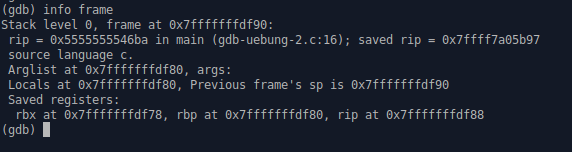
\includegraphics[width=16cm, height=3cm]{Praktikum 2/Bilder/2c_stack_frames2.png}
    \caption{Aufgabe 2c, Info Frame}
\end{figure}
\newpage

\section{Teil 3: GDB Aufgabe 3}
\subsection{Teil A - Analyse des Codes}

Das Skript \textbf{"gdb-uebung-3.c"} enthält eine Funktion f mit return value \textbf{unsigend int} und Übergabeparamter \textbf{unsigned int i} und eine main() Methode. Es wird die Bibliothek \textbf{"stdio.h"} importiert:

\begin{lstlisting}
#include <stdio.h>

unsigned int f(unsigned int i) {
  if (i>1) {
    return i * f(i-1);
  } else {
    return 1;
  }
}

int main() {
  unsigned int i=5, r=0;

  r = f(i);

  printf("i = %d, f(i) = %d\n", i, r);
}
\end{lstlisting}

In der main Methode werden die zwei unsigned Integer Variabeln i \& r mit den Werten 5 \& 0 initialisiert. Im Anschluss wird der Variable r der Rückgabewert der Funktion f mit dem Übergabeparameter i zugewiesen.\\
In der Funktion f wird zunächst geprüft ob i größer eins ist. Falls nicht, wird der das Programm mit einem "return 1" beendet. Andernfalls wird das Programm rekursiv aufgerufen, und i wird bei jedem Aufruf um 1 verringert, bis die Bedingung i > 1 nicht mehr erfüllt ist. Dann werden die Rückgabewerte der Rekursionsaufrufe jeweils mit i multipliziert und am Ende wieder an die main() zurückgegeben. Im Prinzip berechnet f also die Fakultät einer Zahl 1.\\
Durch printf in der main Methode wird der Anfangswert von i, mit dem f aufgerufen wurde, sowie das Ergebnis r ausgegeben.
Es sollte für i=5 und für r=5*4*3*2*1 = 120 (Fakultät von 5) ausgegeben werden.
\newpage


\subsection{Teil B - Kompilieren des Programms}

Das Ergebnis ist wie erwartet:

\begin{figure}[htbp]
    \centering
    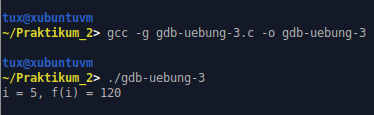
\includegraphics[width=10cm]{Praktikum 2/Bilder/3b_run_script.png}
    \caption{Aufgabe 3b, Ergebnis}
\end{figure}

\subsection{Teil C - Disassembly}

\begin{itemize}
  \item Wie viele Stack Frames werden erzeugt?
\end{itemize}

Es werden Insgesamt sechs Stack Frames erzeugt. Die main() Methode hat einen Frame (\#5) und für jeden rekursiven Aufruf der Funktion f wird ein Frame (\#0 bis \#4) mit dem aktuellen i erzeugt (siehe Abbildung):

\begin{figure}[htbp]
    \centering
    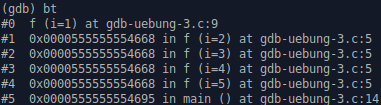
\includegraphics[width=16cm]{Praktikum 2/Bilder/3c_6_stack_frames.png}
\end{figure}

\newpage

\begin{itemize}
  \item Was ist der Inhalt dieser Stack Frames?
\end{itemize}

Der Inhalt besteht aus dem Parameter i der rekursiven Funktion (siehe Abbildung).
\begin{figure}[htbp]
    \centering
    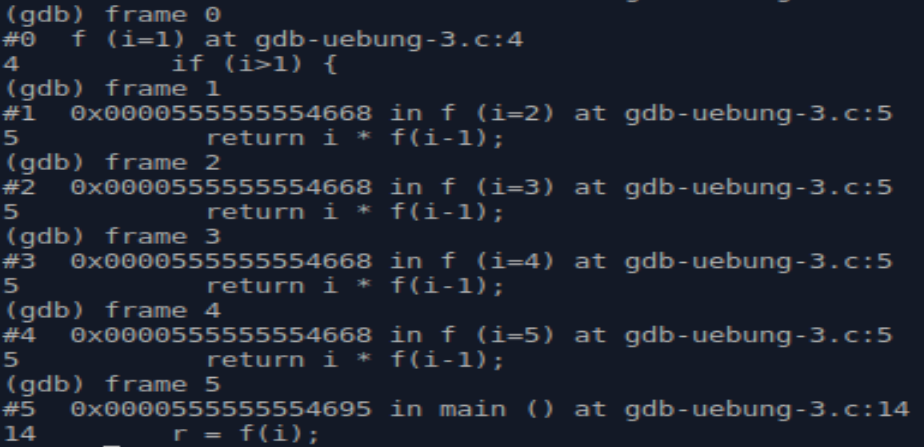
\includegraphics[width=16cm]{Praktikum 2/Bilder/3c_inhalt_der_frames.PNG}
\end{figure}

\begin{itemize}
  \item Wie wird die Parameterübergabe in Assembler umgesetzt?
\end{itemize}

Die System V AMD64 ABI wird unter Linux, FreeBSD und macOS befolgt. Somit ist dies ein Standard unter Unix und Unix-ähnlichen Betriebssystemen. Die ersten sechs Ganzzahl oder Zeigerargumente werden in den Registern: RDI, RSI, RDX, RCX, R8, R9 übergeben. Für Gleitkommazahlen werden folgende Register verwendet: XMM0 bis XMM7.

\newpage

\section{Teil 4: GDB Aufgabe 4}
\subsection{Teil A - Analyse des Codes}
Das Skript \textbf{"gdb-uebung-4.c"} enthält eine nur eine main() Methode.\\
Durch eine for-Schleife sollen die Variablen \textbf{summe} und \textbf{anzahl} berechnet werden. Die Variable i hat einen Wert von 1000. Es soll bei jedem Schleifendurchlauf der Wert 0.01 zur Variable summe addiert werden. Wenn i den Wert 1000.04 erreicht, soll das Programm mit einem "return 0" beendet werden. Demnach sollten es vier Schleifendurchläufe geben.

\begin{lstlisting}
#include <stdio.h>

int main() {
    int anzahl;
    float summe;
    float i;

    summe = 0, anzahl = 0;
    for (i = 1000; i <= 1000.03; i += .01) {
        summe += i;
        anzahl++;
    }
    printf("Summe: %f, Anzahl: %d\n", summe, anzahl);

    return 0;
}
\end{lstlisting}
\subsection{Teil B - Kompilieren des Programms}

Das Ergebnis ist nicht wie erwartet:

\begin{figure}[htbp]
    \centering
    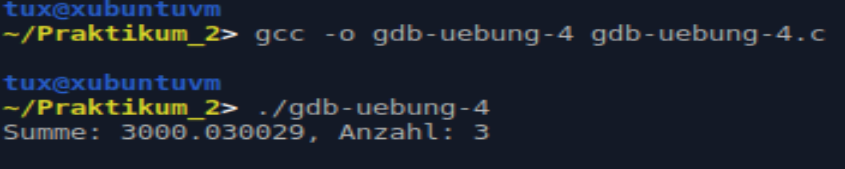
\includegraphics[width=10cm]{Praktikum 2/Bilder/4b_durchlauf.PNG}
    \caption{Aufgabe 4b, Ergebnis}
\end{figure}
\newpage

\subsection{Teil C - Disassembly}

\begin{itemize}
  \item Berechnet die Schleife das korrekte Ergebnis?
\end{itemize}
Die Schleife berechnet nicht das korrekte Ergebnis. Da mit dem Datentyp "float" (Fließkommazahlen) gearbeitet wird, ist davon auszugehen dass Rundungsfehler entstehen können. Das richtige Ergebnis sollte 4000.06 sein.

\begin{itemize}
  \item Welche Werte nehmen die Variablen bei der Ausführung des Programms an?
\end{itemize}
Am Anfang ist anzahl=0, summe=0 und i=1000. In den folgenden Abbildungen sind die Werte der Schleifendurchgänge zu sehen.\\\\
Erster Schleifendurchlauf:
\begin{figure}[htbp]
    \centering
    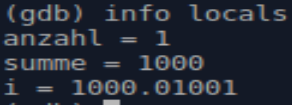
\includegraphics[]{Praktikum 2/Bilder/4c_anzahl_1.PNG}
    \caption{Aufgabe 4c, Teil-Ergebnis}
\end{figure}
\\
Zweiter Schleifendurchlauf:
\begin{figure}[htbp]
    \centering
    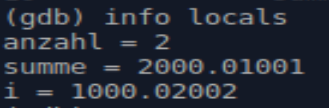
\includegraphics[]{Praktikum 2/Bilder/4c_anzahl_2.PNG}
    \caption{Aufgabe 4c, Teil-Ergebnis}
\end{figure}
\\
Dritter Schleifendurchlauf:
\begin{figure}[htbp]
    \centering
    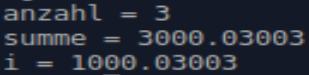
\includegraphics[]{Praktikum 2/Bilder/4c_anzahl_3.PNG}
    \caption{Aufgabe 4c, Ergebnis}
\end{figure}
\\
\begin{itemize}
  \item Warum wird das falsche Ergebnis berechnet?
\end{itemize}
Durch die Bedingung i <= 1000.03 müsste die Schleife ein viertes mal ausgeführt werden, sobald i den Wert 1000.03 erreicht. Durch den Überlauf-Rundungsfehler ist jedoch i > 1000.03, und die Schleife wird kein viertes mal ausgeführt. Dadurch wird die letzte Addition nicht vorgenommen, und der richtige Wert kommt somit nicht zustande.
\newpage

\subsection{Teil D - GDB}
Sobald der Datentyp "double" anstatt "float" verwendet wird, wird die Schleife genau vier mal ausgeführt und liefert das richtige Ergebnis. Der Grund hierfür ist, dass nun für die Darstellung der Zahlen 64-bit statt 32-bit zur Verfügung stehen und damit genügend Bits, um den bei float entstehenden Überlauf abzufangen.
\begin{lstlisting}

#include <stdio.h>

int main() {
    int anzahl;
    double summe;
    double i;

    summe = 0, anzahl = 0;
    for (i = 1000; i <= 1000.03; i += .01) {
        summe += i;
        anzahl++;
    }
    printf("Summe: %f, Anzahl: %d\n", summe, anzahl);

    return 0;
}
\end{lstlisting}
Der Vergleich von Gleitkommazahlen kann wie in der Aufgabe dargestellt nicht immer Funktionieren. Das liegt konkret an der Berechnung von float Werten. Jede Variable des Typs float besteht aus einem Vorzeichenbit, einigen Bits die den Exponenten repräsentieren und Bits die die Mantisse darstellen. Dadurch kann float keine beliebigen realen Zahlen speichern, da diese mit einer Formel berechnet werden müssen. Zum Beispiel würde der Wert 0.1 als 0.100000001490116119384765625 dargestellt werden, das dem 0,1 nächstliegenden 32-Bit Gleitkommawert entspricht. Deshalb ist vom Datentyp float abzuraten sobald es um Nachkommastellen vergleiche geht!
\newpage

\section{Teil 5: GDB Aufgabe 5}
\subsection{Teil A - Analyse des Codes}
Das Skript \textbf{”gdb-uebung-5.c”} besitzt eine binarysearch() Methode die sich rekursiv aufruft und eine main() Methode. Im Prinzip such die binarysearch() nach einem Element (Übergabeparameter "Zahl"). Bei jedem Durchlauf der Methode wird die Rekursiontiefe um eins erhöht und in die Varialbe "rekursiontiefe" gespeichert. Innerhalb der Methode gibt es vier verschiedene Möglichkeiten:\\

\textbf{1.} Wenn die übergebene "Zahl" gleich dem Wert der Stelle "mitte" ist, wird der Wert von "mitte"           zurückgegeben.\\

\textbf{2.} Falls die Werte "links" und "rechts" im Binärbaum dem gleichen Wert entsprechen, wird der Wert "-1"     zurückgegeben.\\ Dadurch wird folgendes ausgegeben: "Zahl \$zahl nicht gefunden!" \\

\textbf{3.} Falls der Wert von "mitte" echt größer ist als die übergebene "Zahl", wird die Methode Rekursiv mit     den gleichen Werten erneut aufgerufen.\\

\textbf{4.} Falls der Wert von "mitte" nicht echt größer ist als die übergebene "Zahl", wird ebenfalls die         Methode Rekursiv aufgerufen, jedoch wird hier für den "links" Paramter der Wert von "mitte"           genommen.\\\\
Der main() Methode wird ein Integer Wert argc, und ein Zeiger auf die Kommandozeilenparamter (argv) in einem Array mitgegeben. In der nächsten Zeile wird geprüft, ob weniger als zwei Parameter übergeben worden sind. Falls dies zutrifft, gibt das Programm eine Ausgabe aus, und beendet das Programm mit "return 1".\\
In Zeile 30 wird der zweite Übergabeparameter (argv[1]) von einem String in eine Integer Zahl konvertiert durch den Befehl \textbf{atoi} (aus der \textbf{"stdlib.h"} Bibliothek), und in die Integer Variable "Zahl" gespeichert. Im Anschluss kommt eine for-Schleife, die solange i kleiner als die Anzahl des Arrays ist, eine Ausgabe macht.\\
Als letztes wird durch eine If else Abfrage eine Ausgabe ausgegeben. Falls die Position größer gleich 0 ist, wird die gesuchte Zahl und die Position im Array ausgegeben. Andernfalls wird ausgegeben, dass die Zahl nicht gefunden wurde. Durch ein \textbf{"return 0"} wird das Programm beendet.
\newpage

\begin{lstlisting}
#include <stdio.h>
#include <stdlib.h>

#define MAX 8 
int array[MAX] = {1,4,12,18,26,31,40,42};
int rekursionstiefe = 0;

int binarysearch(int zahl, int links, int rechts) {
    rekursionstiefe++;
    int mitte = (links + rechts) / 2;
    printf("\nRekursionstiefe: %d", rekursionstiefe);
    if (array[mitte] == zahl)
        return mitte; 
    if (links == rechts)
        return -1; 
    if (array[mitte] > zahl)
        return binarysearch(zahl, links, mitte); 
    else
        return binarysearch(zahl, mitte, rechts);
}

int main(int argc, char *argv[]) {
  int zahl, position, i;
    if(argc < 2) {
        printf("Benutzung: %s <zu suchende Zahl>\n", argv[0]);
        return 1;
    }
    zahl = atoi(argv[1]);

    for (i = 0; i < MAX; i++) {
        printf("%4d", array[i]);
    }
    position = binarysearch(zahl, 0, 7); 
    if (position >= 0) {
        printf("\nGesuchte Zahl %d an Arrayposition %d\n", 
                                            zahl, position);
    }
    else {
        printf("\nZahl %d nicht gefunden\n", zahl);
    }
    return 0;
}
\end{lstlisting}
\newpage

\subsection{Teil B - Kompilieren des Programms}
Bei den Werten 1, 4 und 26 liefert das Programm die entsprechenden Werte. Bei den Werten 27 und 42 endet das Programm in einer Endlosschleife und liefert eine Fehlermeldung:\\

\begin{figure}[htbp]
    \centering
    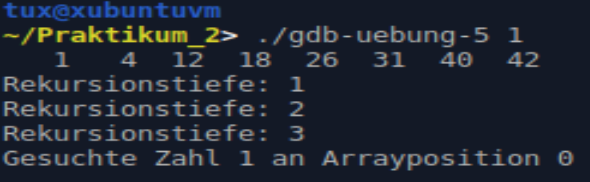
\includegraphics[width=9cm]{Praktikum 2/Bilder/5c_1.PNG}
    \caption{Aufruf mit dem Parameter 1}
\end{figure}

\begin{figure}[htbp]
    \centering
    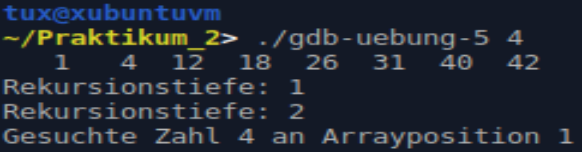
\includegraphics[width=9cm]{Praktikum 2/Bilder/5c_4.PNG}
    \caption{Aufruf mit dem Parameter 4}
\end{figure}

\begin{figure}[htbp]
    \centering
    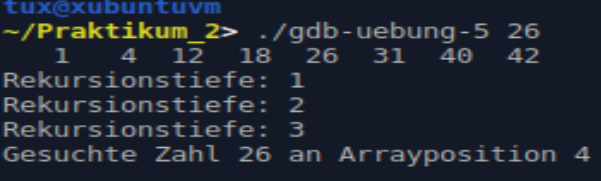
\includegraphics[width=9cm]{Praktikum 2/Bilder/5c_26.PNG}
    \caption{Aufruf mit dem Parameter 26}
\end{figure}

\begin{figure}[!ht]
    \centering
    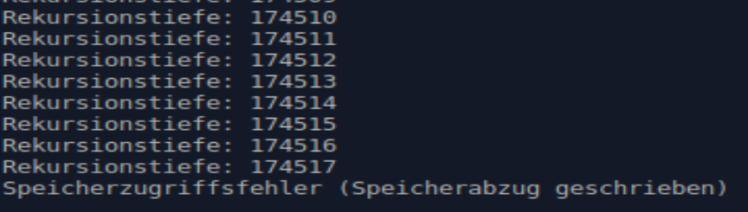
\includegraphics[width=9cm]{Praktikum 2/Bilder/5c_27.PNG}
    \caption{Aufruf mit dem Parameter 27}
\end{figure}

\begin{figure}[!ht]
    \centering
    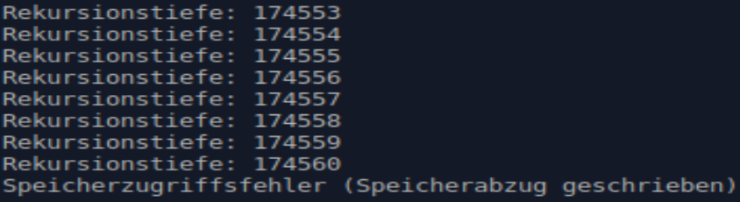
\includegraphics[width=9cm]{Praktikum 2/Bilder/5c_42.PNG}
    \caption{Aufruf mit dem Parameter 42}
\end{figure}
\newpage

\subsection{Teil C - Disassembly}

\begin{itemize}
  \item An welcher Stelle liegt eine fehlerhafte Programmierung vor?
\end{itemize}

In der letzten If-Schleife.\\\\
Die Werte für links und rechts werden im \textbf{else} Block zurückgesetzt, sobald die Variable "mitte = 0" erreicht und der Knoten kleiner ist als die Zahl. Andersherum, wenn die Zahl gleich dem Maximum Knoten entspricht vergleicht Sie die Zahlen nicht und es entsteht ebenfalls eine Endlosschleife.

\begin{itemize}
  \item Aus welchem Grund bricht das Programm ab?
\end{itemize}

Für jeden Funktionsaufruf wird ein Stack Frame angelegt (siehe Abbildung):

\begin{figure}[htbp]
    \centering
    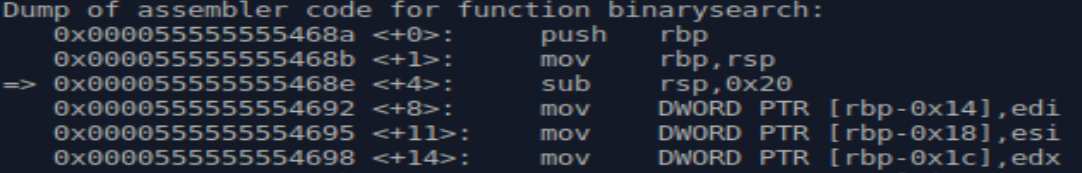
\includegraphics[width=16cm]{Praktikum 2/Bilder/5c_register.PNG}
     \caption{Aufgabe 5c, Stack Frames}
\end{figure}

 Falls die Funktion nun in einer Endlosschleife hängt, werden unendlich viele Stack Frames erstellt. Folglich läuft der reservierte Speicher für das Programm voll. Sobald das Programm kein Speicher mehr zu Verfügung hat, bricht das Programm mit einem "Speicherzugriffsfehler" ab. 
\newpage

\subsection{Teil D - GDB}

Das Original Programm hat folgende Fälle nicht geprüft:

\begin{itemize}
    \item Ob die gesuchte Zahl zwischen zwei Knoten liegen würde, aber nicht existiert.
    \item Ob die gesuchte Zahl gleich dem Wert des maximal Knotens entspricht.
    \item Ob die gesuchte Zahl größer ist als der Wert des maximal Knotens.
\end{itemize}

Um das Programm simpel wie möglich zu halten, wurden die bestehenden Abfragen um weitere If-else Abfragen erweitert. Die entsprechenden If-else Abfragen wurden für den unteren und oberen Bereich des Arrays implementiert und natürlich mit verschiedenen Werten getestet.\\

\begin{lstlisting}
int binarysearch(int zahl, int links, int rechts) {
    rekursionstiefe++;
    int mitte = (links + rechts) / 2;
    printf("\nRekursionstiefe: %d", rekursionstiefe);
    if (array[mitte] == zahl)
        return mitte; 
    if (links == rechts)
        return -1; 
    if (array[mitte] > zahl)                        //untere Knoten
        //Wert liegt zwischen 2 Knoten, ist aber nicht im Array
        if(array[mitte-1] < zahl) 
            return -1;
        else 
                return binarysearch(zahl, links, mitte); 
    else                                            //obere Knoten
        //Zahl ist gleich Max-Knoten
        if(array[rechts] == zahl)
            return rechts;
        //Zahl ist größer Max-Knoten
        else if (array[rechts] < zahl)
            return -1;
        else
            //Wert liegt zwischen 2 Knoten, ist aber nicht im Array
            if(array[rechts-1] < zahl)
                return -1;
            else
                return binarysearch(zahl, mitte, rechts);
}
\end{lstlisting}
\end{document}

%%% Local Variables: 
%%% TeX-PDF-mode: t
%%% TeX-master: t
%%% coding: utf-8
%%% mode: latex
%%% TeX-engine: xetex
%%% End: